\section{Scheduling}

\textbf{Was ist Scheduling?}
\begin{itemize}
	\item Zuordnung von Aufträgen (\textbf{Jobs}) zu Arbeitsträgern, z.B. Maschinen, unter Beachtung von Nebenbedingungen zum Optimieren einer oder mehrerer Zielgrößen
\end{itemize}
\bigskip
\textbf{Scheduling Notation:}
\begin{itemize}
	\item $n$ \textbf{Jobs} müssen auf $m$ \textbf{Maschinen} bearbeitet werden
	\item Job $j$ hat auf Maschine $i$ eine \textbf{Prozesszeit} $p_{ij}$
	\item Job $j$ kann ein \textbf{Gewicht} $w_j$ haben $\rightarrow$ Repräsentiert die Wichtigkeit des Jobs
	\item Job $j$ kann einen \textbf{Liefertermin} $d_j$ haben
	\item Notation eines \textbf{Scheduling-Problems}: $\alpha\mid\beta\mid\gamma$
	\begin{itemize}
		\item $\alpha$: Maschinenumgebung
		\item $\beta$: Auftragscharakteristik und Beschränkungen
		\item $\gamma$: Zielgröße
	\end{itemize}
\end{itemize}
\bigskip
\textbf{Performanz-Kenngrößen:}
\begin{itemize}
	\item \textbf{Fertigstellungszeitpunkt (Completion Time) $\boldsymbol{C_j}$}:
	\begin{itemize}
		 \item Zeitpunkt, zu welchem Job $j$ fertiggestellt ist
		 \item Bei mehreren Maschinen $C_{ij}$ (Fertigstellung von Job $j$ auf Maschine $i$) gilt: $C_j=\max\limits_{i\in I}\{C_{ij}\}$
	\end{itemize}  
	\item \textbf{Unpünktlichkeit (Lateness)} $L_j=C_j-d_j$ beschreibt die Abweichung vom Fertigstellungszeitpunkt zum Liefertermin. Negativ, wenn Produkt zu früh fertig
	\item \textbf{Verspätung (Tardiness)} $T_j=\max\{C_j-d_j,0\}$ wie Lateness, aber erlaubt keine negativen Werte
	\item \textbf{Einheits-Strafe (Unit penalty)}  
	$U_j=
	\begin{cases}
		1\;, & \text{wenn } C_j > d_j\\
		0\;, & \text{sonst}
	\end{cases}$
	\newline
	\newline
	erhebt eine Einheitsstrafe, wenn Fertigstellungszeitpunkt zu spät
\end{itemize}
\bigskip
\textbf{Maschinenumgebung $\boldsymbol{(\alpha)}$:}
\begin{itemize}
	\item \textbf{Einzel Maschine} $\boldsymbol{(1)}$
	\item \textbf{Parallele Maschinen $\boldsymbol{(Pm, Qm, Rm)}$:}
	\begin{itemize}
		\item Mehrere Maschinen, die gleichzeitig Jobs abarbeiten
		\item $Pm$: $m$ identische Maschinen (gleiche Geschwindigkeit)
		\item $Qm$: $m$ Maschinen mit unterschiedl., job-unspezifischen Geschwindigkeiten
		\item $Rm$: $m$ Maschinen mit unterschiedl., job-spezifischen Geschwindigkeiten
	\end{itemize}
	\item \textbf{Flow-Shop $\boldsymbol{(Fm)}$}: $m$ Maschinen in Serie, alle Jobs müssen diese durchlaufen (selbe Maschinen-Reihenfolge)
	\item \textbf{Job-Shop $\boldsymbol{(Jm)}$}: $m$ Maschinen, alle Jobs müssen diese durchlaufen, haben jedoch unterschiedliche Maschinen-Reihenfolge
\end{itemize}
\bigskip
\textbf{Auftragscharakteristik $\boldsymbol{(\beta)}$:}
\begin{itemize}
	\item \textbf{Freigabezeiten (Release dates) $\boldsymbol{(r_j)}$}: Auftrag kann nicht vor diesem Zeitpunkt gestartet werden
	\item \textbf{Unterbrechungen (Preemptions) $\boldsymbol{(prmp)}$}: Bearbeitung eines Auftrags kann unterbrochen und später fortgesetzt werden
	\item \textbf{Permutation $\boldsymbol{(prmu)}$}: Job-Reihenfolge auf der ersten Maschine muss beibehalten werden
	\item \textbf{Rüstzeiten (Setup times) $\boldsymbol{(s_{jk}, s_{jk}^i)}$}:
	\begin{itemize}
		\item Bevor mit Auftrag $k$ begonnen werden kann, ist Maschine $i$ durch Umrüstung blockiert
		\item $s_{jk}$: Rüstzeit ist nur von den aufeinanderfolgenden Jobs $j$ und $k$ abhängig
		\item $s_{jk}^i$: Rüstzeit ist zusätzlich von Maschine $i$ abhängig
	\end{itemize}
\end{itemize}
\bigskip
\textbf{Zielfunktion $\boldsymbol{(\gamma)}$:}
\begin{itemize}
	\item \textbf{Makespan $\boldsymbol{(C_{max})}$}: Entspricht Gesamtproduktionszeit, also der Zeit, wenn der letzte Job fertiggestellt ist: $C_{max}=\max\limits_{j\in J}\{C_j\}$
	\item \textbf{Gesamtfertigstellungszeiten (Total completion time) $\boldsymbol{(\sum C_j)}$:} Summe der Fertigstellungszeiten der Jobs
	\item \textbf{Gewichtete Gesamtfertigstellungszeiten (Total weighted completion time) $\boldsymbol{(\sum w_jC_j)}$:} Summe der gewichteten Fertigstellungszeiten der Jobs
	\item \textbf{Gesamtverspätung (Total tardiness) $\boldsymbol{(\sum T_j)}$:} Summe der Verspätungszeiten
	\item \textbf{Anzahl verspäteter Jobs (Number of tardy Jobs) $\boldsymbol{(\sum U_j)}$:} Summe der Einheitsstrafen
\end{itemize}
\bigskip
\textbf{Gantt-Charts:}
\begin{itemize}
	\item Visualisierungsmöglichkeit von Scheduling-Lösungen
	\item Block für die Bearbeitung von Job $j$ auf Maschine $i$ ist auf Höhe von
	$i$ und Länge des Blocks entspricht Prozesszeit $p_{ij}$
	\item Innerhalb des Blocks steht die Job-Nummer oder Prozesszeit (problemabhängig)
\end{itemize}
\begin{center}
	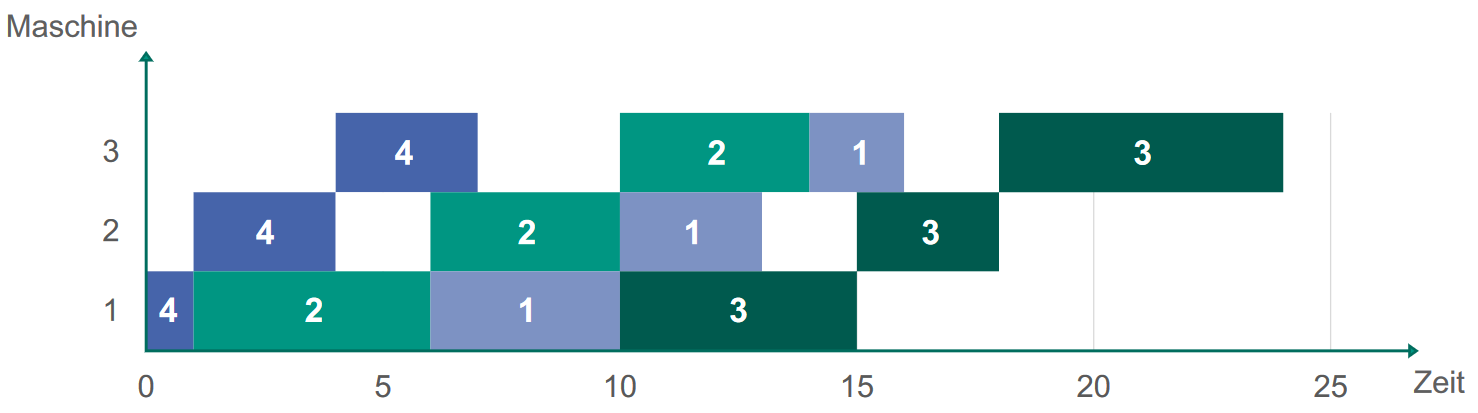
\includegraphics[width=0.7\textwidth]{images/gantt.png}
\end{center}

\subsection{Ein-Maschinen-Probleme}
\begin{itemize}
	\item \textbf{Problemstellung}: $n$ Jobs sollen auf einer Maschine in
	Reihenfolge gebracht werden
	\item Jeder Schedule kann als Permutation der Jobs $1,\ldots,n$ angesehen
	werden \\
	$\rightarrow n!$ verschiedene Schedules
\end{itemize}
\bigskip
\textbf{Minimierung der Fertigstellungszeiten:}
\begin{itemize}
	\item Problem $1\mid\mid C_{max}$ ist trivial, da $C_{max}=\sum\limits_{j=1}^{n} p_j$ für jeden Schedule
	\item Problem $1\mid\mid \sum\limits_{j=1}^{n} C_j$ lässt sich mit \textbf{SPT-Regel} (Shortest Processing Time first) optimal lösen $\rightarrow$ Individuelle Fertigstellungszeitpunkte so gering wie möglich halten
	\begin{center}
		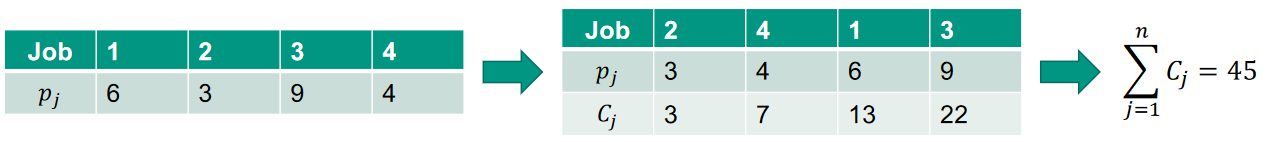
\includegraphics[width=0.8\textwidth]{images/spt.png}
	\end{center}
\end{itemize}
\bigskip
\textbf{Minimierung gewichteter Fertigstellungszeiten:}
\begin{itemize}
	\item Problem $1\mid\mid \sum\limits_{j=1}^{n} w_jC_j$ lässt sich mit \textbf{WSPT-Regel} (Weighted shortest processing time) optimal lösen
	\begin{center}
		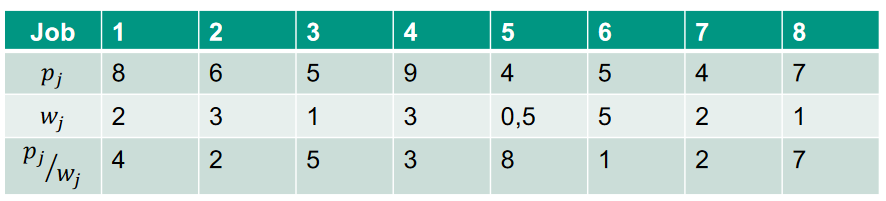
\includegraphics[width=0.7\textwidth]{images/wspt.png}
	\end{center}
	\item Es ergibt sich $S=\{6,2,7,4,1,3,8,5\}$ mit $\sum\limits_{j=1}^{n} w_jC_j(S)=329$
\end{itemize}
\bigskip
\textbf{Minimierung der Anzahl verspäteter Jobs:}
\begin{itemize}
	\item Problem $1\mid\mid \sum\limits_{j=1}^{n} U_j$ lässt sich mit \textbf{Moore's Algorithmus} optimal lösen
	
\end{itemize}
